\section{挑战}
\label{sec:challenges}

脚手架驱动的智能体强化学习改变了训练引擎观察与建模一次 rollout 的方式。在传统智能体 RL 中，训练引擎拥有环境交互循环并维护完整的 token 历史。此处 $p_t$ 表示第 $t$ 步的 prompt token，$a_t$ 表示对应的响应 token，$o_t$ 为 token 化的环境观测。下一步 prompt 构造为
\begin{equation}
  p_t = (p_{t-1},a_{t-1},o_t).
\end{equation}
整个 rollout 遵循序列 $(p_1,a_1,o_1,a_2,o_2,a_3,\ldots)$，构成良定义的马尔可夫过程，自然映射为一条线性训练样本。

在\add{\harl{}}中，脚手架拥有环境交互循环与消息状态，训练引擎只能观察通过 LLM 端点发出的调用。对一次 rollout $\rho$，它记录序列
\begin{equation}
  \mathcal{C}(\rho)
  = \bigl((p_1,a_1),(p_2,a_2),\ldots,(p_{T_\rho},a_{T_\rho})\bigr),
\end{equation}
其中 $p_i$ 为 prompt token，$a_i$ 为模型实际采样的响应 token。这些调用之间的环境交互与脚手架状态转移不可直接观察。因此，将观察到的调用序列组装为训练样本本身成为一个建模问题。这一差异带来了若干实现挑战。现有框架的处理方式各不相同，可能影响算法正确性与训练稳定性。

\add{更形式化地说，传统智能体 RL 与\harl{}都可用部分可观测马尔可夫决策过程（POMDP）刻画，区别在于潜在状态与呈现给策略模型的观测。在\harl{}中，令
\begin{equation}
  s_t = \bigl(s_t^{\mathrm{harness}},s_t^{\mathrm{env}}\bigr)
\end{equation}
表示由脚手架与环境共同维护的潜在执行状态。模型不直接观察 $s_t$；脚手架构造消息级上下文并将其渲染为用于生成的确切 token 级 prompt：
\begin{align}
  C_t^{\mathrm{msg}}
    &= \operatorname{Context}_{H}\bigl(s_t^{\mathrm{harness}}\bigr),\\
  p_t^{\mathrm{tok}}
    &= \operatorname{Tok}\bigl(\operatorname{Template}
       (C_t^{\mathrm{msg}})\bigr).
\end{align}
每个策略决策因此被记录为一次调用级转移
\begin{equation}
  z_t = \bigl(p_t^{\mathrm{tok}},a_t^{\mathrm{tok}}\bigr),
  \qquad
  a_t^{\mathrm{tok}} \sim
  \pi_\theta\bigl(\cdot \mid p_t^{\mathrm{tok}}\bigr).
\end{equation}
一次 rollout 产生变长集合的此类转移，且不假设相邻 prompt 之间存在精确的 token 前缀关系。任何为训练所做的序列构造都必须保留每个动作实际采样时所依据的 prompt。下面描述\harl{}特有的若干新挑战。}

\subsection{重分词与样本合并}

\paragraph{\add{为什么 token 前缀连续性会被破坏。}}

\begin{figure}[t]
  \centering
  \begin{tikzpicture}[
      tok/.style={draw, rounded corners=1pt, minimum height=0.55cm,
        inner sep=2pt, font=\scriptsize, align=center},
      ptok/.style={tok, fill=microsoftcard, draw=microsoftline,
        text width=1.3cm},
      newtok/.style={tok, fill=microsoftcard, draw=microsoftline,
        text width=1.5cm},
      atok/.style={tok, fill=microsoftblue!12, draw=microsoftblue},
      mismatch/.style={tok, fill=red!12, draw=red!70!black},
      rowlabel/.style={font=\scriptsize\bfseries, text=microsoftgray,
        align=left, text width=3.1cm},
    ]
    \node[rowlabel] (labelA) at (0,1.7) {第 $i$ 次调用的实际采样};
    \node[ptok] (pA) at (3.3,1.7) {$p_i^{\mathrm{tok}}$};
    \node[atok, right=1mm of pA] (a1A) {h};
    \node[atok, right=1mm of a1A] (a2A) {aving};
    \draw[decorate, decoration={brace, amplitude=3pt, mirror},
      microsoftblue, thick]
      (a1A.south west) -- (a2A.south east)
      node[midway, yshift=-0.32cm, font=\scriptsize, text=microsoftblue]
      {$a_i^{\mathrm{tok}}$};

    \node[rowlabel] (labelB) at (0,0.3) {$p_{i+1}^{\mathrm{tok}}$ 的直接重分词};
    \node[ptok] (pB) at (3.3,0.3) {$p_i^{\mathrm{tok}}$};
    \node[mismatch, right=1mm of pB] (b1) {hav};
    \node[mismatch, right=1mm of b1] (b2) {ing};
    \node[newtok, right=1mm of b2] (bnew) {新回合};
    \draw[decorate, decoration={brace, amplitude=3pt, mirror},
      microsoftgray, thick]
      (pB.south west) -- (bnew.south east)
      node[midway, yshift=-0.32cm, font=\scriptsize, text=microsoftgray]
      {$p_{i+1}^{\mathrm{tok}}$};

    \node[font=\scriptsize, text=red!70!black, anchor=west]
      at ([xshift=2mm]bnew.east)
      {$\ne a_i^{\mathrm{tok}}$：无法合并};
  \end{tikzpicture}
  \caption{一个重分词示例。第 $i$ 次调用中单词 \texttt{having} 被采样为 \texttt{h} 与 \texttt{aving} 两个 token（\emph{上}）；当更新后的消息历史为第 $i{+}1$ 次调用重新分词时，同一文本可能被切分为 \texttt{hav} 与 \texttt{ing} 的不同 token 边界（\emph{下}）。尽管底层文本相同，token 边界却不同。即使式~\ref{eq:text-prefix} 的文本级前缀条件仍成立，式~\ref{eq:token-prefix} 的 token 级前缀条件也被破坏。}
  \label{fig:retokenization}
\end{figure}

智能体脚手架通常通过文本消息与模型 API 通信。从脚手架视角看，一次 rollout 通常由回合级调用组成
\begin{equation}
  \mathcal{C}^{\mathrm{text}}(\rho)
  = \bigl((p_1^{\mathrm{text}},a_1^{\mathrm{text}}),
  (p_2^{\mathrm{text}},a_2^{\mathrm{text}}),\ldots\bigr),
\end{equation}
其中脚手架发送 $p_i^{\mathrm{text}}$ 并收到 $a_i^{\mathrm{text}}$。典型地，对于多回合 ReAct 式~\cite{react} 智能体，前一次调用构成下一次 prompt 的完整文本级前缀，例如
\begin{equation}
  (p_i^{\mathrm{text}}, a_i^{\mathrm{text}}) \preceq p_{i+1}^{\mathrm{text}}.
  \label{eq:text-prefix}
\end{equation}
此外，当脚手架派生子智能体或摘要压缩上下文时，训练引擎可能收到不满足该关系、拥有不同 prompt 历史的后续调用。

RL 训练基于精确的 token ID 与 rollout 对数概率。RL 系统用 token 序列 $p_i^{\mathrm{tok}}$ 与 $a_i^{\mathrm{tok}}$ 表示每次调用，其中 $a_i^{\mathrm{tok}} \sim \pi_\theta(\cdot \mid p_i^{\mathrm{tok}})$。返回给脚手架的响应为 $a_i^{\mathrm{text}}=\operatorname{Decode}(a_i^{\mathrm{tok}})$。训练因此观察 token 级序列 $\mathcal{C}^{\mathrm{tok}}(\rho)=((p_1^{\mathrm{tok}},a_1^{\mathrm{tok}}), (p_2^{\mathrm{tok}},a_2^{\mathrm{tok}}),\ldots)$。

\add{相邻调用之间的 token 前缀连续性要求
\begin{equation}
  \bigl(p_i^{\mathrm{tok}},a_i^{\mathrm{tok}}\bigr)
  \preceq p_{i+1}^{\mathrm{tok}},
  \label{eq:token-prefix}
\end{equation}
其中 $\preceq$ 表示精确的 token 级前缀关系。}

实践中，式~\ref{eq:text-prefix} 成立并不保证式~\ref{eq:token-prefix} 成立。下一次请求是将聊天模板与分词器应用于更新后的消息历史得到的。重分词后，$p_{i+1}^{\mathrm{tok}}$ 中对应 $a_i^{\mathrm{text}}$ 的 token ID 可能与最初采样于 $a_i^{\mathrm{tok}}$ 的 ID 不同。

\add{我们在研究中观察到这种错配至少由三种机制引起：
\begin{enumerate}[leftmargin=*,label=(\arabic*)]
  \item \textbf{聊天模板的非组合性。}
  渲染完整消息历史不一定等价于拼接各部分的渲染结果：
  \begin{equation}
    \operatorname{Template}(A \mathbin{\Vert} B)
    \ne
    \operatorname{Template}(A)
    \mathbin{\Vert}
    \operatorname{Template}(B).
  \end{equation}
  模板可能在消息边界插入分隔符或连接换行，也可能省略原始生成中出现的标记。实践中我们即发现 Qwen 的聊天模板可能移除早先出现的 \texttt{<think>} 标记，破坏 token 前缀连续性。

  \item \textbf{解码-重分词漂移。}
  token 解码并非单射，将采样 token 转回文本再重新分词未必恢复原始 token ID：
  \begin{equation}
    \operatorname{Tok}
      \bigl(\operatorname{Decode}(a_i^{\mathrm{tok}})\bigr)
    \ne a_i^{\mathrm{tok}}.
  \end{equation}
  图~\ref{fig:retokenization} 给出具体例子：单词 \texttt{having} 在第 $i$ 次调用中被采样为 \texttt{h} 与 \texttt{aving} 两个 token，而在后续 prompt 中重新分词同一文本可能得到 \texttt{hav} 与 \texttt{ing}。尽管解码文本未变，token 边界却不同，破坏了两次调用间的 token 级连续性。

  \item \textbf{推理时的输出变换。}
  工具调用与结构化输出处理器可能在把采样响应返回脚手架之前对其进行解析、规范化、修复与重新序列化。这类处理可能改变空白符、分隔符、JSON 结构或非法语法，因此后续 prompt 中并入的响应即使在文本层面也可能与采样 token ID 所代表的响应不同。
\end{enumerate}}

\paragraph{\add{缓解被破坏的 token 前缀连续性。}}

\add{最直接的策略是独立训练每次模型调用：每个生成 token 视为其所属调用的动作的一部分，损失在 $(p_i^{\mathrm{tok}},a_i^{\mathrm{tok}})$ 上计算，不假设与相邻调用的任何关系。这保证 token 级正确性，但计算低效——跨调用共享的长 prompt 前缀被重复计算。不同框架用不同策略处理。}

AReaL~\cite{areal2} 与 verl Uni-Agent~\cite{uniagent} 在 LLM 代理中维护请求缓冲区，保存每次调用的历史文本与 token。新请求到达且其文本与缓冲历史精确匹配时，框架用缓冲的响应 token 替换新 prompt token 中对应上一响应文本的片段，保证 token 前缀条件恒成立。slime~\cite{slime} 与 Polar~\cite{polar} 不做此替换。

\add{这种替换不止恢复计算复用：当缓冲 token ID 与实际下一次请求中的不同时，它改变了评估下一次响应所依据的 prompt。假设实际下一次 prompt 包含上一响应的重构版本 $\widehat{a}_i^{\mathrm{tok}}$：
\begin{equation}
  p_{i+1}^{\mathrm{tok}}
  =
  p_i^{\mathrm{tok}}
  \mathbin{\Vert}
  \widehat{a}_i^{\mathrm{tok}}
  \mathbin{\Vert}
  \Delta_{i+1}.
\end{equation}
将该片段替换为最初采样的 $a_i^{\mathrm{tok}}$ 得到拼接 prompt
\begin{equation}
  \widetilde{p}_{i+1}^{\mathrm{tok}}
  =
  p_i^{\mathrm{tok}}
  \mathbin{\Vert}
  a_i^{\mathrm{tok}}
  \mathbin{\Vert}
  \Delta_{i+1},
  \qquad
  \widetilde{p}_{i+1}^{\mathrm{tok}}
  \ne p_{i+1}^{\mathrm{tok}}.
\end{equation}
响应 $a_{i+1}^{\mathrm{tok}}$ 采样自以 $p_{i+1}^{\mathrm{tok}}$ 为条件的策略，而非以 $\widetilde{p}_{i+1}^{\mathrm{tok}}$ 为条件。在拼接 prompt 下训练它因此引入离线（off-policy）偏差。精确 token 前缀重叠仅应在保留 rollout 实际消耗的 prompt 时用于合并。}

\add{第二种方法是前缀共享或树形结构训练。精确的共同 token 前缀只表示一次，分支感知的因果注意力掩码确保 token 只关注其祖先与同分支上更早的 token。这可以复现独立训练因果序列的结果，同时复用前缀计算。然而，树打包、自定义注意力掩码或 kernel、切分以及分布式梯度处理需要大量训练后端支持。}

\add{第三种实用方法是尽力而为的序列合并。两次相邻调用仅在其观测 token ID 满足式~\ref{eq:token-prefix} 时合并：条件成立时只追加未匹配的后缀与下一动作；不成立时关闭当前序列并开启新序列。这保留了 rollout 期间消耗的 prompt，并可与标准稠密因果 kernel 配合，重分词漂移只会降低合并率。Agent Lightning v1.0 采用此策略，作为独立调用重算与后端密集的树形训练之间的折中。}

\add{这些方法各有权衡。缓冲 token 替换可提高合并率，但一旦改变 rollout 实际消耗的 prompt 就变成离线拼接。独立调用训练与尽力而为合并保证 token 级正确性，但可能遗留冗余前缀计算；树形结构训练可回收更多复用，代价是后端显著复杂。}

\subsection{优势计算}
\label{subsec:advantage-calculation}

LLM 调用合并后，一次 rollout $\rho$ 可产生不同数量的训练样本 $N_\rho$，该数量只有在执行与样本构建之后才能确定。重分词是这种动态样本数的一个来源；脚手架还可能派生子智能体——产生不共享单一线性历史的分支——或摘要压缩上下文，用新的 token 前缀替换旧前缀。这些操作可将一次任务级 rollout 拆分为多个训练样本。这并非边缘情形：在我们的编程智能体训练中（图~\ref{fig:smith-merge-sample-metrics}），平均仅 36\% 的 rollout 保持为单一训练样本，每次 rollout 平均产生 2.4 个训练样本。

实践中，奖励仍基于最终结果，并分配给产生该结果的 rollout 内的每个样本。这引出一个自然问题：计算优势时，组统计量应在 rollout 层面还是样本层面计算？我们发现现有框架选择各异：verl Uni-Agent~\cite{uniagent} 与 Polar~\cite{polar} 在 rollout 层面计算优势，而 slime~\cite{slime} 与 AReaL~\cite{areal2} 在样本层面计算。

图~\ref{fig:rollout-sample} 给出具体例子。假设 Rollout 1 与 Rollout 2 由同一 prompt 在一个 GRPO~\cite{deepseekmath} 组内生成，Rollout 1 获得奖励 1，Rollout 2 获得奖励 0。在传统 RL（\emph{左}）中，每次 rollout 恰好映射为一个训练样本，基线 $\bar{r}=(1+0)/2=1/2$ 没有争议。在\add{\harl{}}（\emph{右}）中，Rollout 1 有三个样本（Sample 1、Sample 2、Sample 3），Rollout 2 只有一个样本（Sample 4）：rollout 级优势计算的基线仍为 $\bar{r}_{\mathrm{rollout}}=(1+0)/2=1/2$，而样本级优势计算给出 $\bar{r}_{\mathrm{sample}}=(1+1+1+0)/4=3/4$。

\begin{figure}[t]
  \centering
  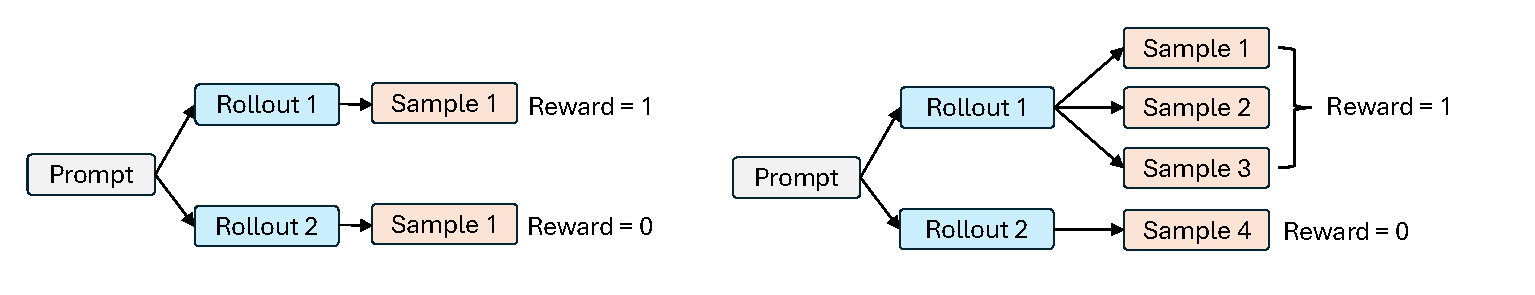
\includegraphics[width=\linewidth]{figures/agl-lite-reward.pdf}
  \caption{传统智能体 RL 中每次 rollout 是一个训练样本（\emph{左}），对比\add{\harl{}}中一次 rollout 可展开为继承其奖励的动态数量样本（\emph{右}）。}
  \label{fig:rollout-sample}
\end{figure}

我们认为 rollout 级优势是更合理的选择，理由如下。重分词是偶发现象，优势分配不应仅仅因为重分词恰巧把一次 rollout 拆成更多样本而改变。同理，子智能体派生与上下文摘要压缩是脚手架的内部操作，不应被允许改变整个组的基线。如何在一次 rollout 的样本之间设计更好的信用分配，仍有待未来工作。

\subsection{损失归一化}
\label{subsec:loss-normalization}

动态样本数也使损失归一化成为不平凡的选择。考虑一个包含 $R$ 次 rollout 的训练批次，其中 rollout $\rho$ 产生 $N_\rho$ 个样本，rollout $\rho$ 的第 $j$ 个样本有 $L_{\rho,j}$ 个响应 token，逐 token 损失为 $\ell_{\rho,j,t}$（$t=1,\ldots,L_{\rho,j}$）。多数框架直接沿用传统智能体 RL 的样本级归一化。第一种是 DAPO~\cite{dapo} 使用的 token 均值损失，对批次内所有 token 求和并按响应 token 总数归一化：
\begin{equation}
  \mathcal{L}_{\mathrm{token\text{-}mean}}
  = \frac{\sum_{\rho=1}^{R}\sum_{j=1}^{N_\rho}\sum_{t=1}^{L_{\rho,j}}
    \ell_{\rho,j,t}}
    {\sum_{\rho=1}^{R}\sum_{j=1}^{N_\rho} L_{\rho,j}}.
  \label{eq:token-mean}
\end{equation}
第二种是 GRPO~\cite{deepseekmath} 使用的序列均值-token 均值损失，先在每个样本内取均值，再对所有样本的样本均值均匀平均：
\begin{equation}
  \mathcal{L}_{\mathrm{seq\text{-}mean}}
  = \frac{1}{\sum_{\rho=1}^{R} N_\rho}
    \sum_{\rho=1}^{R}\sum_{j=1}^{N_\rho}
    \frac{1}{L_{\rho,j}}\sum_{t=1}^{L_{\rho,j}} \ell_{\rho,j,t}.
  \label{eq:seq-mean}
\end{equation}
slime~\cite{slime} 实现了 rollout 级 token 均值损失，先将一次 rollout 的所有响应 token 汇总，再在 rollout 之间均匀平均：
\begin{equation}
  \mathcal{L}_{\mathrm{rollout\text{-}mean}}
  = \frac{1}{R}\sum_{\rho=1}^{R}
    \frac{\sum_{j=1}^{N_\rho}\sum_{t=1}^{L_{\rho,j}} \ell_{\rho,j,t}}
    {\sum_{j=1}^{N_\rho} L_{\rho,j}}.
  \label{eq:rollout-mean}
\end{equation}

我们在图~\ref{fig:loss-normalization} 中给出更具体的例子。假设一个批次包含三次 rollout：Rollout A 产生两个样本 $A_1$ 与 $A_2$，响应长度分别为 50 与 100；Rollout B 产生三个样本 $B_1$、$B_2$ 与 $B_3$，每个响应长度 30；Rollout C 产生单个样本 $C_1$，响应长度 40。令 $A_1,A_2,B_1,B_2,B_3,C_1$ 同时表示各样本内逐 token 损失之和，即 $A_1=\sum_t \ell_{A,1,t}$，以此类推。则：
\begin{itemize}
  \item $\mathcal{L}_{\mathrm{token\text{-}mean}}
  = (A_1+A_2+B_1+B_2+B_3+C_1)/(50+100+30+30+30+40)$。
  \item $\mathcal{L}_{\mathrm{seq\text{-}mean}}
  = \tfrac{1}{6}(A_1/50+A_2/100+B_1/30+B_2/30+B_3/30+C_1/40)$。
  \item $\mathcal{L}_{\mathrm{rollout\text{-}mean}}
  = \tfrac{1}{3}\bigl((A_1+A_2)/(50+100)+(B_1+B_2+B_3)/(30+30+30)+C_1/40\bigr)$。
\end{itemize}

\begin{figure}[t]
  \centering
  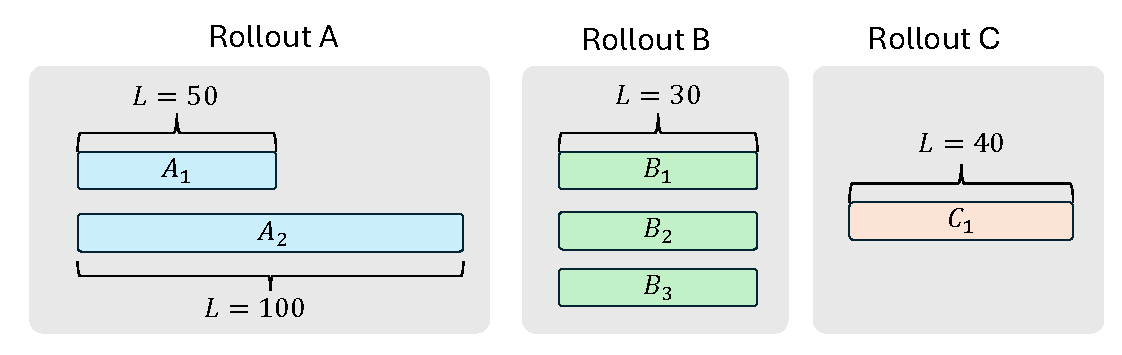
\includegraphics[width=0.65\linewidth]{figures/agl-lite-rollout-sample.pdf}
  \caption{一个包含三次 rollout、样本数与响应长度各异的示例批次。}
  \label{fig:loss-normalization}
\end{figure}

对损失归一化，我们持与优势计算相同的观点：样本数量不应被允许影响梯度归一化，因为它常由重分词等偶然因素驱动。在此观点下，式~\ref{eq:seq-mean} 的序列均值-token 均值损失是有问题的：它随单个 rollout 恰好产生的样本数而变化，总体上给样本更多的 rollout 不成比例的高权重。因此我们认为式~\ref{eq:token-mean} 的 token 均值损失与式~\ref{eq:rollout-mean} 的 rollout 级 token 均值损失在理论上更合理。但实践中我们发现 token 均值损失对长序列敏感：当批次中出现许多长负样本时，可能在训练后期引发不稳定。因此我们偏好式~\ref{eq:rollout-mean} 的 rollout 级 token 均值损失。

\subsection{训练后端复杂度}

动态样本数也使与训练后端的接口复杂化。一批 rollout 的样本数量与长度只有在脚手架执行与样本构建之后才能确定；相比之下，训练 GPU 数量与数据/张量/流水线并行配置在整个训练期间通常保持固定。后端因此必须在每次迭代将可变负载映射到固定 worker 集合上。

\add{样本构建之后，后端可将结果序列展平为物理张量批次，但这一变换必须保留其统计来源。尤其地，每条序列都应保留其 rollout 标识与 prompt 组标识：
\begin{equation}
  \mathcal{B}_{\mathrm{train}}
  =
  \bigcup_{\rho \in \mathcal{B}_{\mathrm{rollout}}}
  \left\{
    \bigl(S_{\rho,j},\rho,g_\rho\bigr)
    \;\middle|\;
    1 \le j \le N_\rho
  \right\},
\end{equation}
其中 $S_{\rho,j}$ 是由 rollout $\rho$ 构造的第 $j$ 条序列，$g_\rho$ 标识由同一 prompt 采样的一组 rollout。展平只改变物理表示，不得改变 rollout 归属，也不得让某次 rollout 仅仅因为产生了更多序列而获得额外统计权重。}

\add{rollout 边界还约束批次调度。基于行的张量批次、数据并行切分与小批次调度无法仅凭 prompt 或 rollout 数量提前规划，因为 $N_\rho$ 只有在执行后才知道。此外，同一次 rollout 的序列应保持在同一次优化器更新中——把它们拆分到不同更新中，会让一次 rollout 的不同部分在不同策略版本下被评估，引入 rollout 内策略偏差。后端因此必须在固定 worker 之间平衡 token 负载，同时保留这些 rollout 级统计与更新边界。}
